\section{Monopolio}
\begin{itemize}
    \item Neoclásica: monopolios pueden surgir de la manera de legislación y por monopolios naturales. 
    \item Austriaca: solo hay un monopolista, los creados por el gobierno. Ejemplo Maycom.
\end{itemize}

%----------------------------------------------------------------------------------------
\section{\pregunta{Cuáles son las fuentes de PODpoder de mercado} }
\begin{itemize}
    \item Patentes 
    \item Licencias de exclusividad 
    \item Economías de escala 
    \item Derecho exclusivo a un input 
    \item Innovaciones tecnológicas
\end{itemize}

%----------------------------------------------------------------------------------------
\section{\pregunta{En qué punto un monopolista maximiza sus ganancias} }
\begin{itemize}
    \item Nivel de output en el que \textbf{Ingreso marginal = costo marginal}
        \begin{itemize}
            \item Empresa competitiva: ingreso marginal = precio, esto no aplica para el monopolista. 
        \end{itemize}
    
    \item Un monopolista no posee una pequeña parte del mercado. Ya que vende un bien o servicio único, enfrenta la curva de demanda en su plenitud. 
    
    \item Para el monopolio el ingreso marginal es menor al precio: $\displaystyle IM < P$ 
\end{itemize}
\begin{figure}[H]
    \centering
    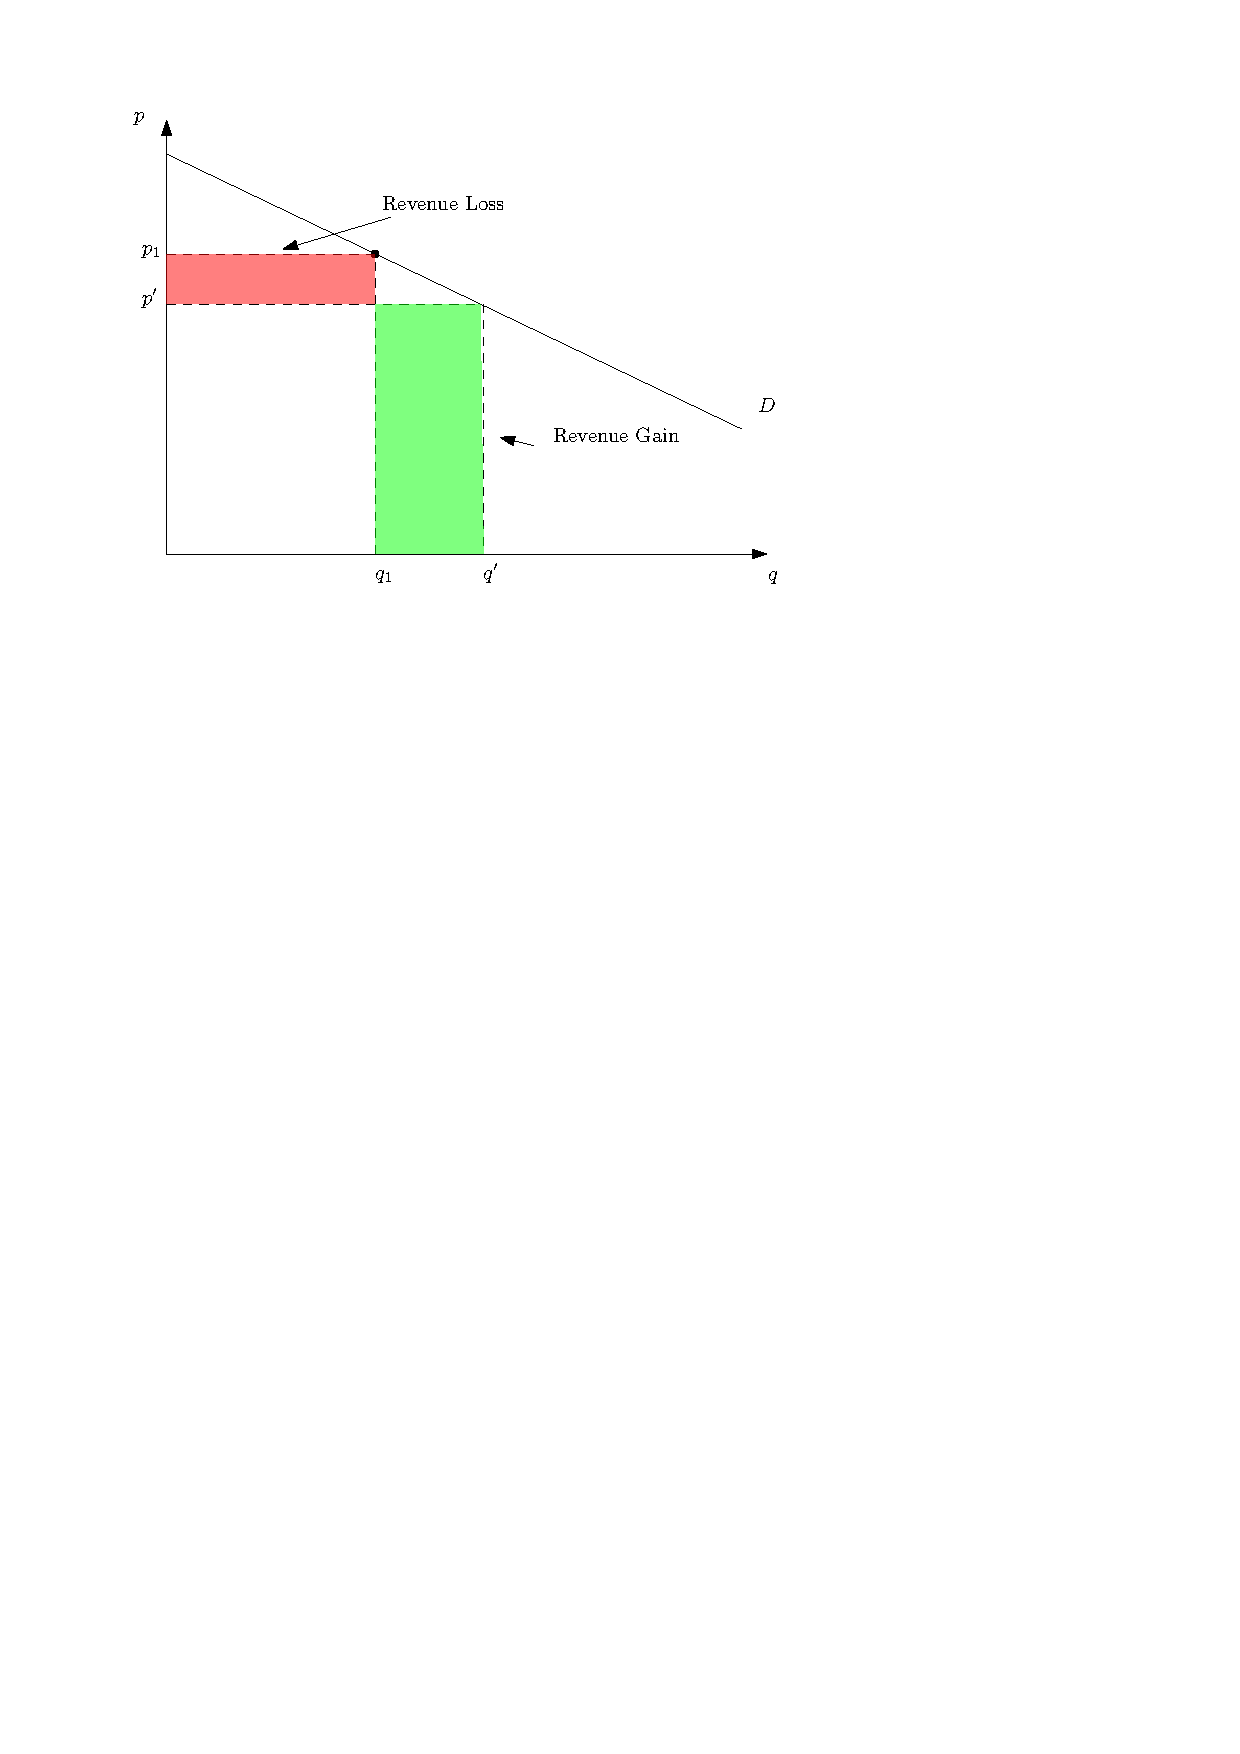
\includegraphics[]{Clases/figs/monopoly} 
\end{figure}
\begin{itemize}
    \item Dado a que es un bien único esto permite poder poner el precio mucho más caro que el costo. 
\end{itemize}

\section{Eligiendo precio o cantidad...}
{A diferencia de una empresa competitiva, un monopolio puede ajustar precio o cantidad para maximizar ganancias, pero está limitado por la demanda del mercado (no puede elegir un precio y cantidad por encima de la curva de demanda).
} \newline 


\section{\pregunta{Cómo calcular el ingreso marginal} }
\begin{itemize}
    \item Maximizamos ganancias cuando precio marginal es igual al ingreso marginal.
\end{itemize}

\begin{figure}[H]
    \centering
    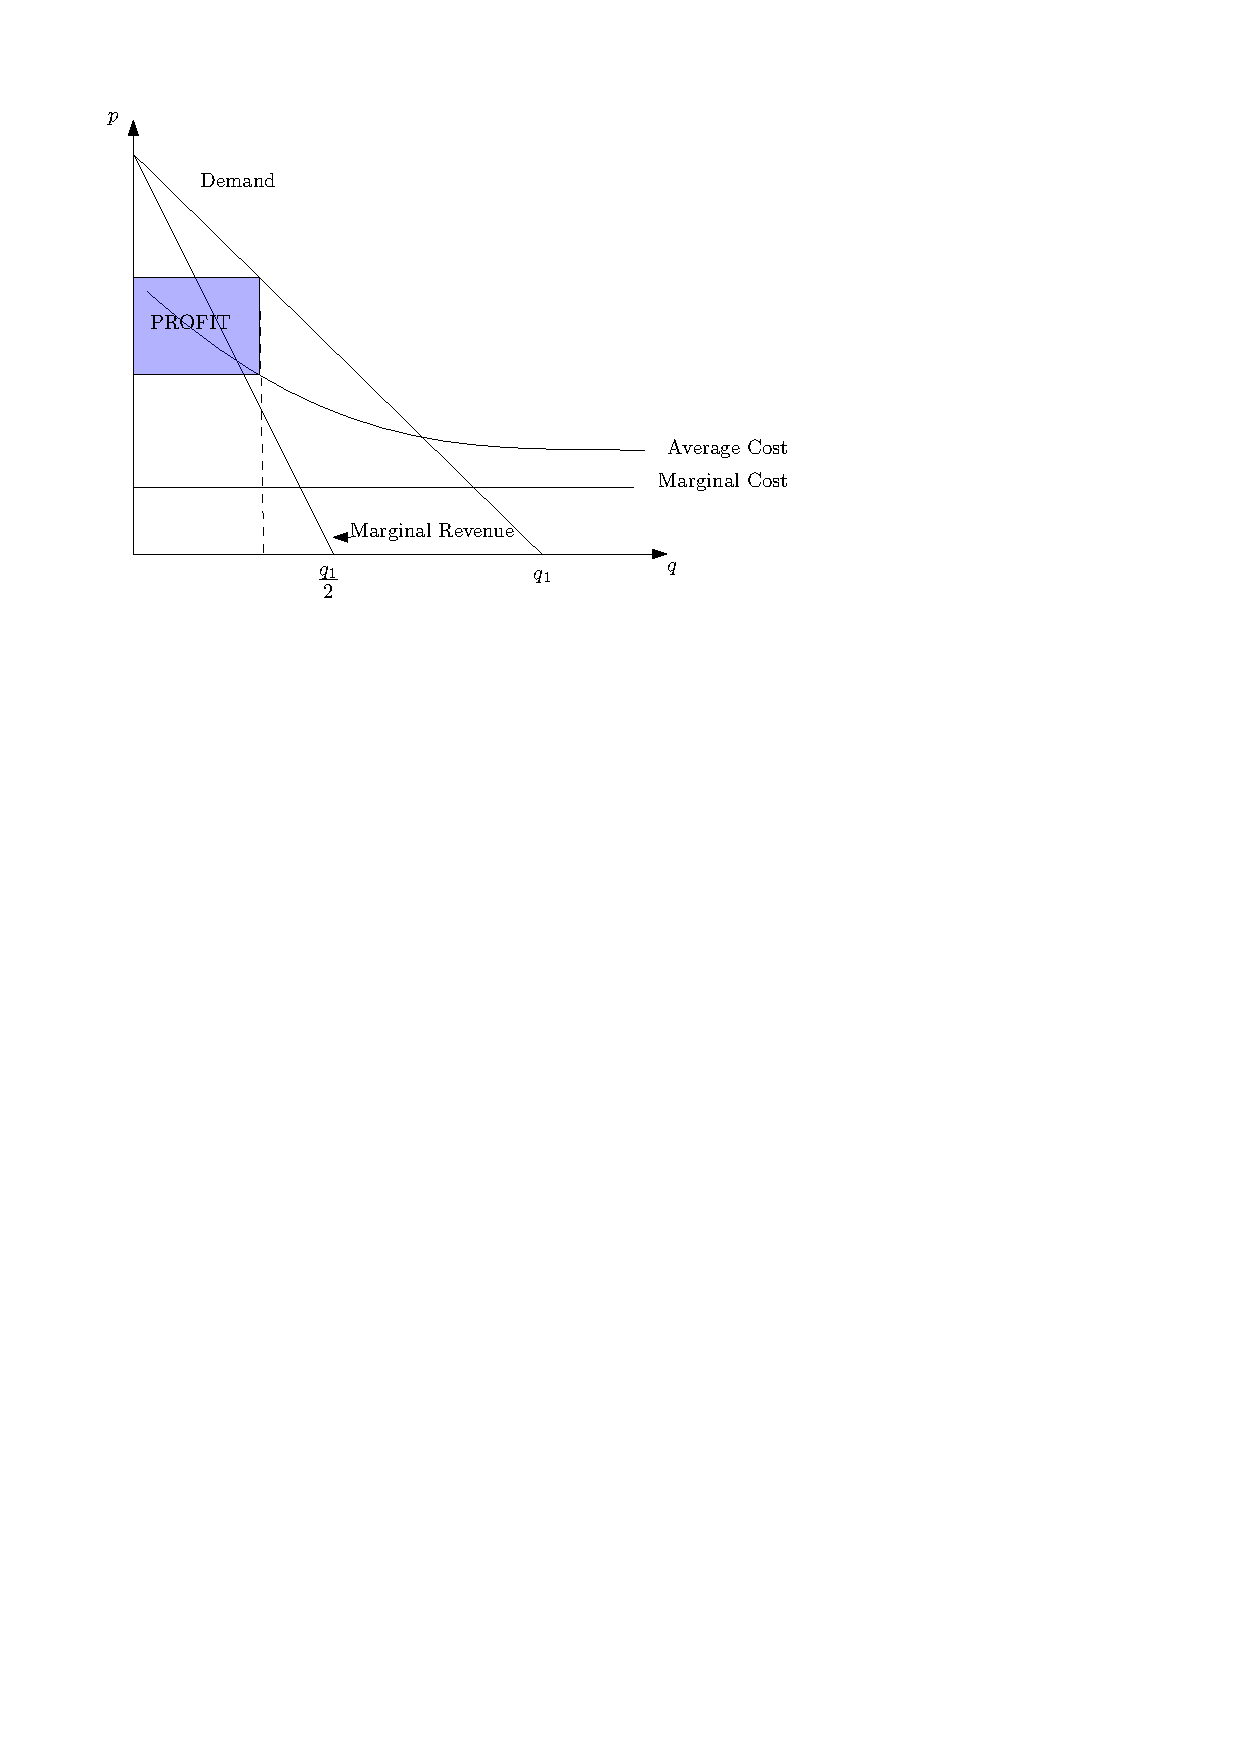
\includegraphics[]{Clases/figs/profit} 
\end{figure}




%----------------------------------------------------------------------------------------
\section{Markup}
\termdefinition{Markup}{Qué tanto puede poner el monopolista el precio por encima del costo marginal} 

\begin{figure}[H]
    \centering
    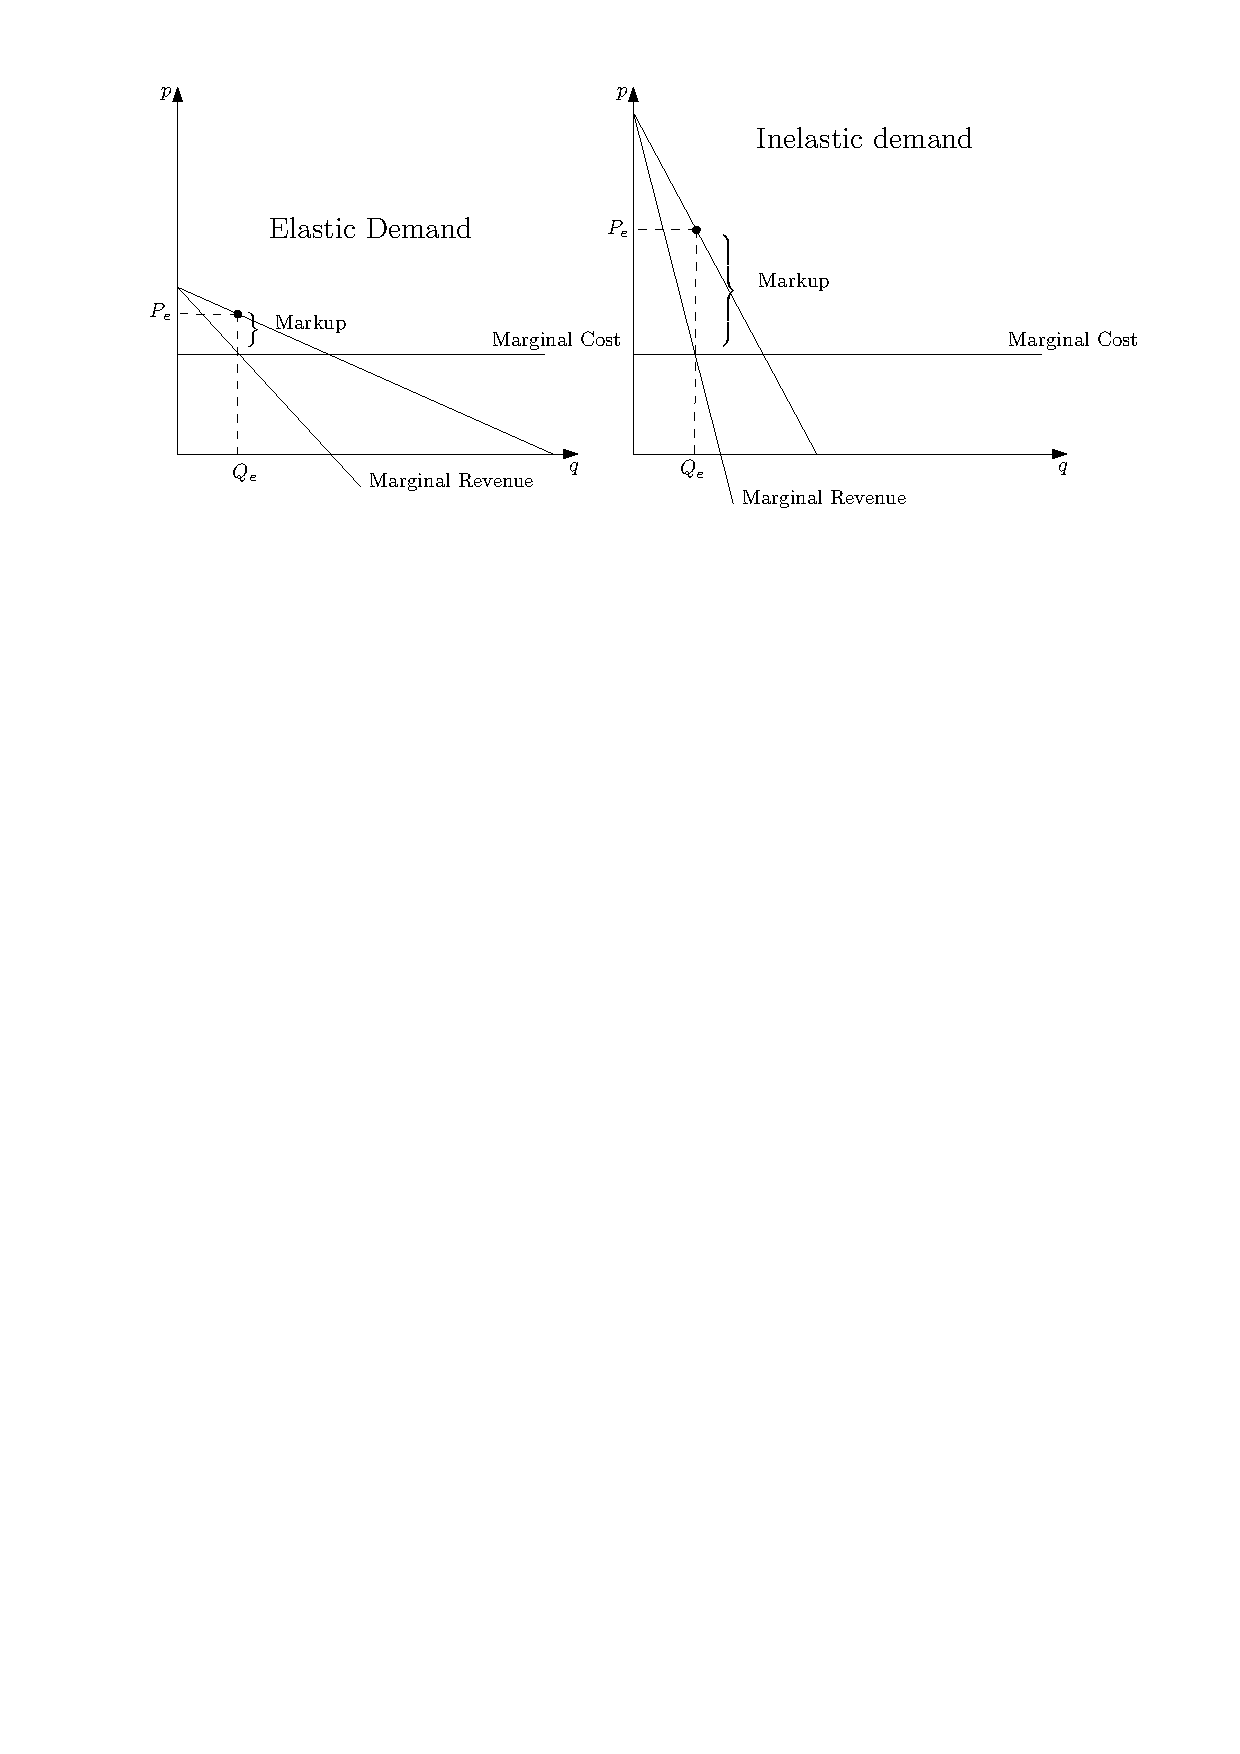
\includegraphics[]{Clases/figs/markup} 
\end{figure}


%----------------------------------------------------------------------------------------
\section{Learner}
El tamaño del markup:
\[
  L = \frac{P-MC}{P} 
\]
\[
  L = \frac{P-MC}{P} = \frac{1}{\left| E \right| } 
\]



%----------------------------------------------------------------------------------------
\section{Ejercicio}
\begin{center}
   \begin{align*}
       P &= 100 - 2Q \\ 
       CF &= 100 \\ 
       CM &= 20 \\ 
   \end{align*}
   Encontrar Q*, P*, Ingresos totales y ganancias ($\pi $) Graficar.
   \begin{align*}
       \text{ Encontrar el marrginal Revenue:  } \\ 
       IM &= 100 - \underbrace{4}_{\times 2}  Q \\ 
       \text{ igualamos IM = CM para encontrar Q*.  } \\ 
       100 - 4 Q &= 20 \\ 
        Q* &= \frac{1}{4} \p{80} \qimplies 20 \\  
        \text{ Encontrar P* } \\ 
        P* &= 100 - 2\p{20} \qimplies 60 \\ 
        \text{ Encontrar los ingresos totales y costos totales: } \\ 
        IT &= P \times Q = 20 \times 60 = 1200 \\ 
        CT &= CF + CV = CF + CM \times Q = 100 + 20 \p{20} = 500 \\ 
        \text{ Hallar las ganancias (profits) } \\ 
        \pi &= IT - CT = 1200 - 500 = 700 \\ 
   \end{align*}
   \begin{figure}[H]
       \centering
       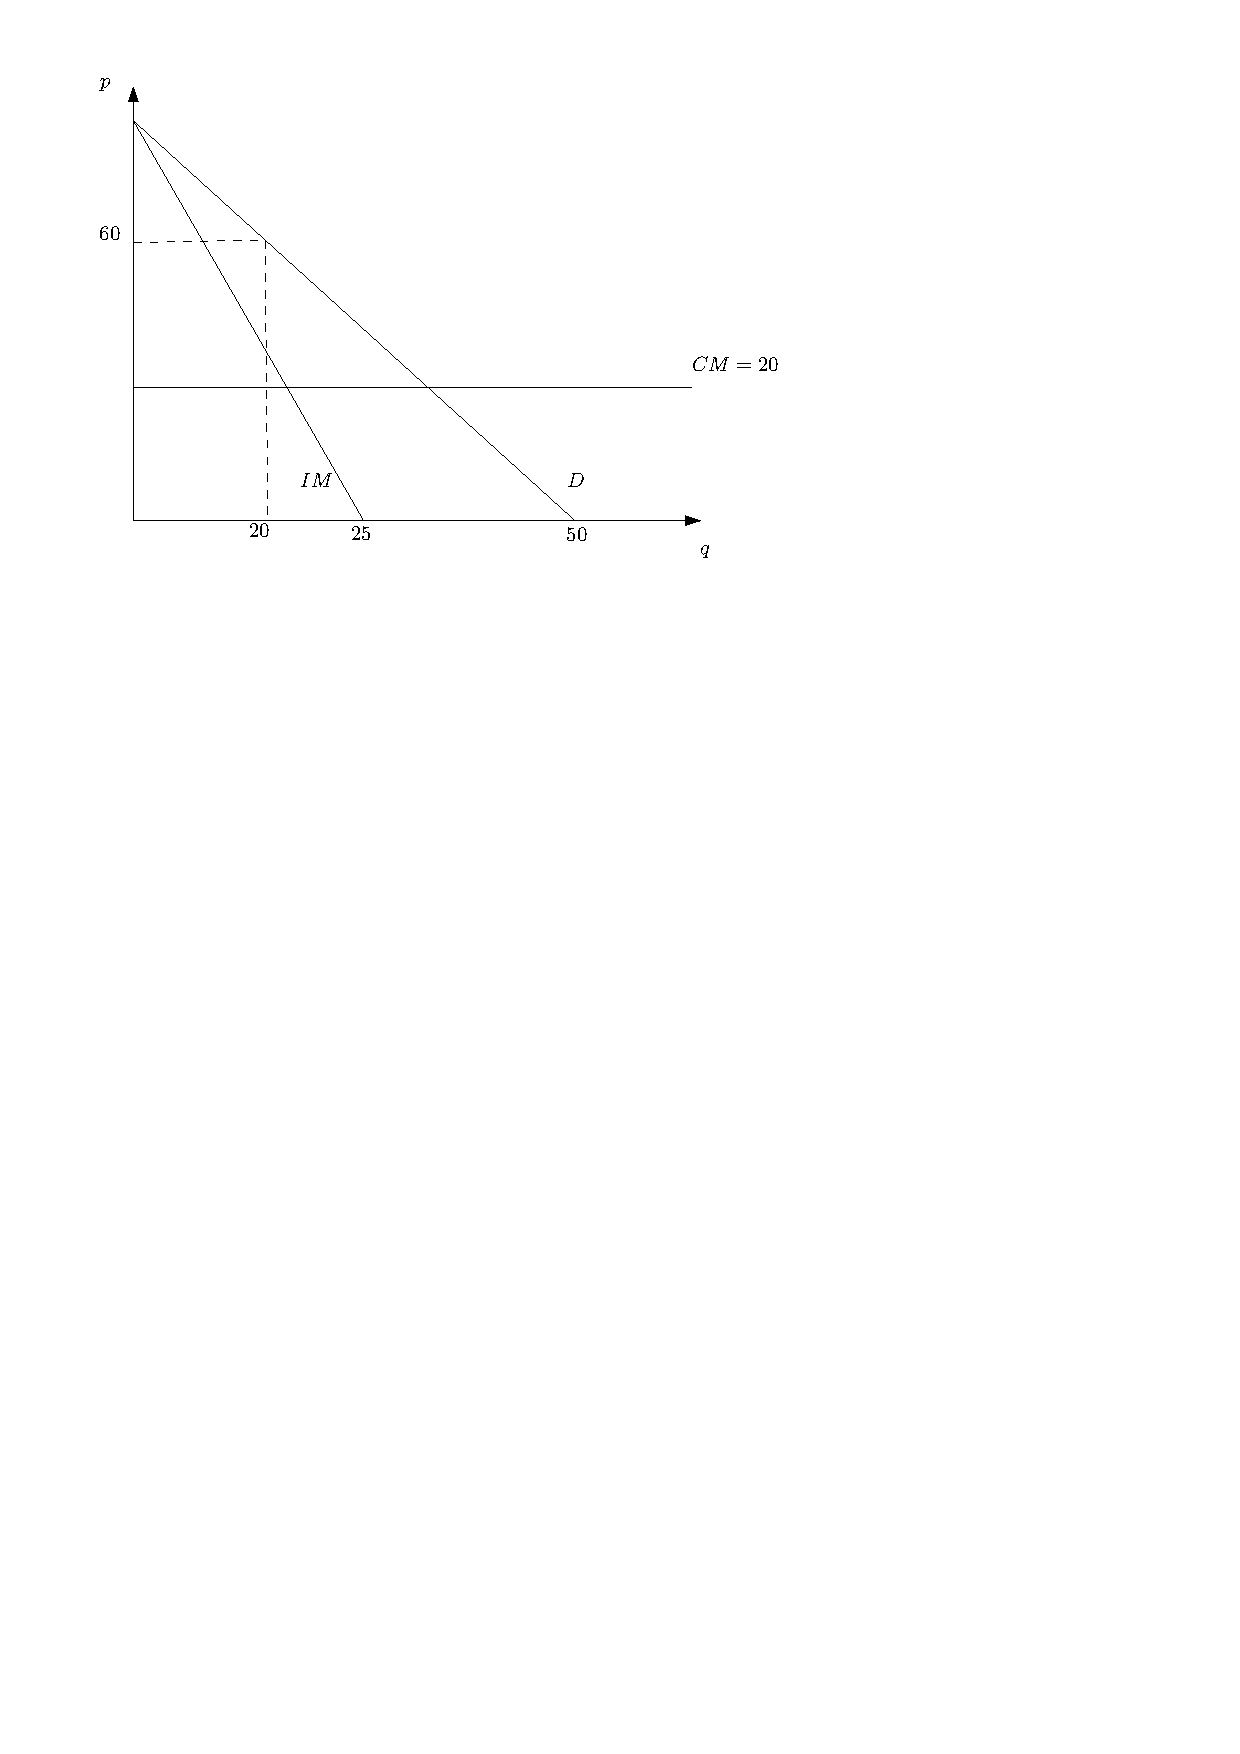
\includegraphics[]{Clases/figs/ejercicio} 
   \end{figure}
\end{center}
